\section{Examples}

\subsection{Multi-drone path planning}\label{sec:Multirobot}

Every drone is modeled as a control system $\Sigma^i=(X,x_\init^i,U,W,f^d_\tau)$, 
where $f^d_\tau$ is the sampled-time abstraction of the following continuous dynamics:
\begin{equation*}\label{eq:unicycle_ss}
	f^{d}(x(t),u(t)) :=
	\begin{bmatrix}
		\dot{x}_1\\
		\dot{x}_2\\
		\dot{x}_3
	\end{bmatrix}=
	\begin{bmatrix}
		u_1cos(x_3)\\
		u_1sin(x_3)\\
		u_2
	\end{bmatrix}.
\end{equation*}
where $x_1$ and $x_2$ denote the drone's position \MZ{(Meter)} in two-dimensional space, $x_3$ denotes the rotational angle \MZ{(Radian)}, and $u_1$ and $u_2$ represent control inputs for each drone. Choosing a sampling time $\tau=0.1s$, the nominal dynamics $f^d_\tau$ can be characterized uniquely. 
We consider state and input spaces to be $X=[-1,11]^2\times[-2,3.3]$ and $U=[-2.4,2.4]^2$, respectively. 
The disturbance set and robustness margin are chosen as $|W|\leq (0,0.025,0.025)$ and $\varepsilon=(0.20,0.20,0.24)$.

Recall that we consider 10 drones, i.e., $N = 10$.
Selecting the horizon length $T=104$ and minimum safe distance $\delta=0.24$, ALTRO computes a valid open-loop trajectory 
in $77.8$ seconds for the product system with $30$ state and $20$ input variables.  
Fig.~\ref{fig:3dtubes} gives time-space illustration for the safe tubes around the nominal trajectories. 

For ABCD, we set  $\eta_{X}=(0.025,0.025,0.03)$ and $\eta_{U}=(0.3,0.3)$. 
Tab.~\ref{tab:runtimes} shows the run times and number of state-input pairs corresponding to both local and global ABCD. 
Noticeably, already when $N=2$, memory requirement for global ABCD exceeds memory limits, 
even 1.5TB RAM on a cluster machine is not sufficient to synthesize a controller.

On the other hand, using ALTRO alone would not provide guarantee against bounded disturbance.  
Fig.~\ref{fig:multi_drone_distance} illustrates the performance of open-loop and feedback controllers in regulating distance between two particular 
the drones with and without disturbances. 
As expected, in the absence of disturbances, the open-loop controllers suffice and the distance between the two drones (shown in solid blue) 
does not go below the defined threshold. 
Next, we consider the case when constant additive disturbances $(0 ,0.025,0.025)$ 
and $(0,-0.025,-0.025)$ are being applied to the two drones throughout the whole horizon. 
It can be noticed that applying the open-loop controller causes that distance between the two drones (shown in solid yellow) to 
go below the predefined threshold. 
However, the feedback controller is capable of maintaining distance (shown in solid red) within the safe region when the same disturbance is being applied.


%In this example, we are focusing on number of robots. This example consist of 10 identical unicycle model. Each unicycle should start from its own initial point and reach target set which is shown in Fig. \ref{fig:MA} with green points and red points. while it avoids obstacles and collision with other agents. Unicycle model is described in below.
%\begin{equation}\label{eq:unicycle_ss}
%	f^{u}(x(t),u(t))=
%	\begin{bmatrix}
%	\dot{x_1}\\
%	\dot{x_2}\\
%	\dot{x_3}
%	\end{bmatrix}=
%	\begin{bmatrix}
%	u_1cos(x_3)\\
%	u_1sin(x_3)\\
%	u_2
%	\end{bmatrix}.
%\end{equation}
%In Eq. \ref{eq:unicycle_ss} $u_1$ is linear speed and $u_2$ is  angular speed and $x_1$ and $x_2$ represents positions and $x_3$ is the angle. Here goal of the problem is designing a controller which satisfy the specifications which mentioned in sec. \ref{sec:Problem_statement}. For this purpose, According to sec.\ref{sec:nominal trajectory} at first we combine all of unicycle dynamics to create a centralized model of the centralized system. The centralized system has $10\times3$ dimension for state space and $10\times2$ dimension for input space. For collision avoidance and obstacle avoidance we use $\delta_{col}=1.5$ and $\delta_{obs}=2$ and we use euclidean distance as a metric for distance in 2D space. In this step, we solved mentioned problem with ALTRO with sample time 0.05 and 200 points for trajectory. Computation takes 138 seconds. Result of ALTRO is illustrated in fig \ref{fig:MA}. 
%In next step we synthesize close loop controller using ABCD with $\varepsilon=[0.16,0.16,0.16]$.  As we mentioned in Prob. \ref{alg:abcd-with-time-for-tracking} we are going to to design a controller that is able to track the trajectory with $\varepsilon$ distance in every time step which is also robust to the disturbance .\MZ{Here we can split the centralized system to 10 separate system and design a close loop controller for each one of them separately.} In order to do this step, we select $\varepsilon$ in a way that it satisfies $\delta_{col} > 2\sqrt{\varepsilon_x^2+\varepsilon_y^2}$ (since tubes should not intersect with each other). Then we are able to design a controller guaranteeing the specifications for each agent independently using Alg. \ref{alg:abcd-with-time-for-tracking} and SCOTS. We select parameters in this way:\\
%$\widetilde{X}=[-1:11]*[-1:11]*[-\pi,\pi]*[0,1]$\\
%$U=[-3,3]*[-3,3]$\\
%$\eta_{\widetilde{X}}=[0.04,0.04,0.04,0.05]$\\
%$\eta_{U}=[0.6,0.6]$\\
%number of states = about $7*10^7$\\
%reduced number of states = about $7*10^7$\\
%number of inputs =121\\
%
%Abstraction in total for 10 systems takes about 12 minutes(average 100 seconds for each system) and synthesizing controller takes about 2 minutes(near 15 seconds for each system). Controller designed in this way is able to overcome bounded additive disturbance $|w|\leq[0.03,0.03,0.03]$ (for all of unicycles). Nominal controller which is produced by ALTRO with presence of this disturbance will be pushed outside of $\epsilon$ tube and also as it shown in the Fig.\ref{fig:MA}, trajectory 1 and 2 will have collision with this value of disturbance. 




 %Figure~\ref{fig:inv_pend} demonstrates variations of disturbance limit under which SCOTS is able to find a controller for different tube width. %It can be observed that by increasing the tube width, SCOTS is able to synthesize a controller for larger disturbance levels. Figure~\ref{fig:invpend_traj} demonstartes trajectories of the system  \eqref{eq:inv_pend_ssq} governed by controllers synthesized by ALTRO and SCOTS under appliance of constant disturbance vector \MS{$[??,??]$}. As expected, the controller designed by ALTRO is not able to tackle disturbance, while using the controller generated by SCOTS, the trajectory remains within the desired bound.

%\begin{figure}\label{fig:inv_pend}
%	\includegraphics[]{}
%	\caption{Variations of disturbance limit for which SCOTS is able to find a controller with tube size}
%\end{figure}
%\begin{figure}\label{fig:invpend_traj}
%	\includegraphics[]{}
%	\caption{}
%\end{figure}
%\textcolor{red}{

\begin{figure}[t]
	\centering
	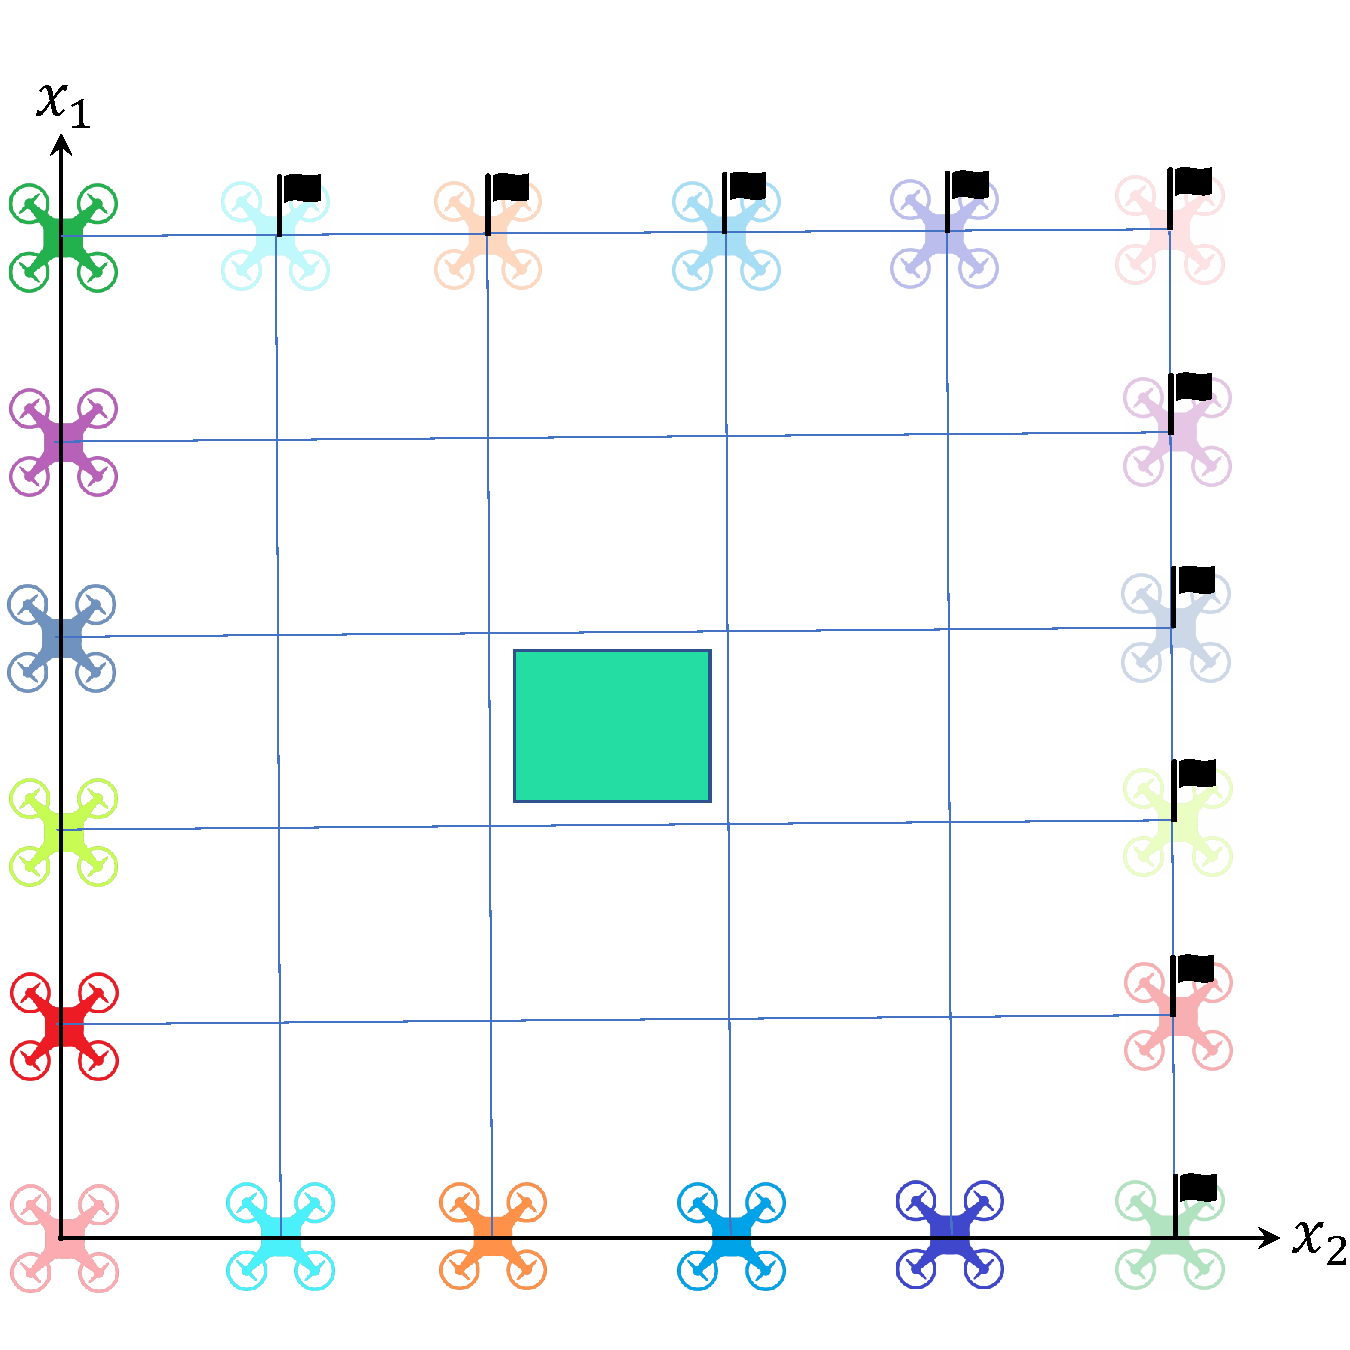
\includegraphics[width=.2\textwidth]{figures/multidrone.pdf}
	\caption{The mission map for the multi-drone path planning example}
	\label{fig:MA}
\end{figure}
\begin{figure}[t]
	\centering
	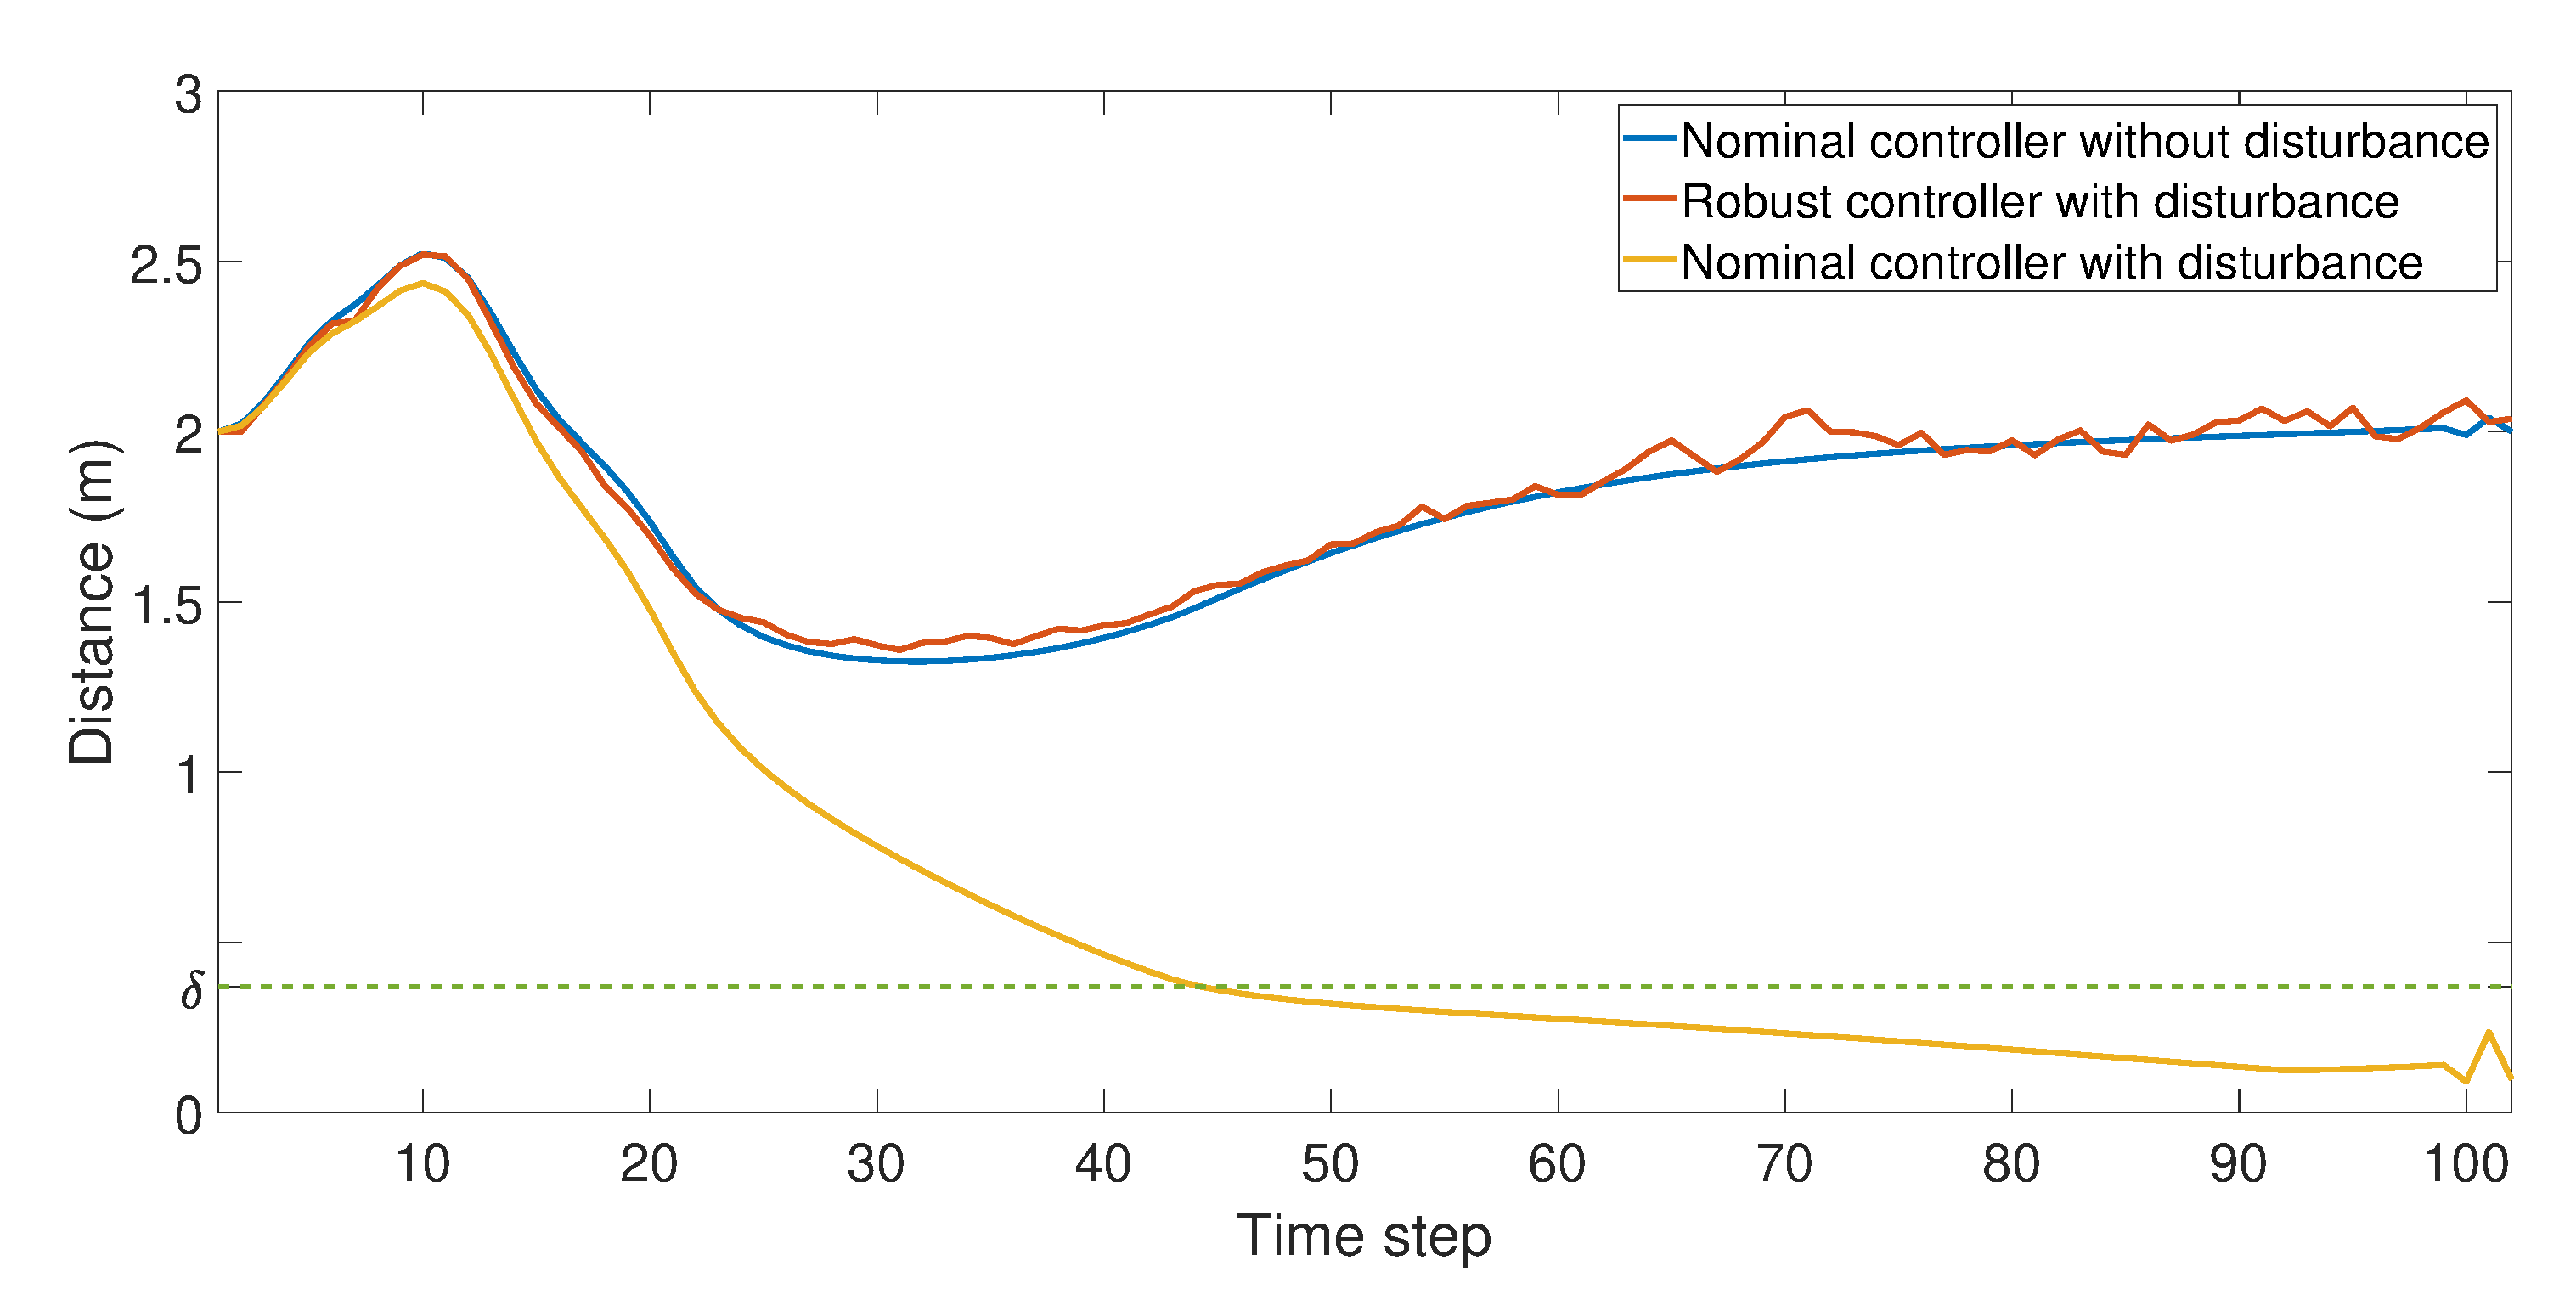
\includegraphics[width=.4\textwidth]{figures/multi_drone2.eps}
	\caption{Performance of open-loop and feedback controllers in regulating distance between two selected drones for disturbance-free and perturbed situations for the multi-drone path planning example}
	\label{fig:multi_drone_distance}
\end{figure}

\subsection{Crane and Vehicle}
\label{subsec:crane_vehicle}
We model the crane and vehicle as control systems 
$\Sigma^1=(X^1,x_\init^1,U^1,W^1,f_\tau^c)$ and $\Sigma^2=(X^2,x_\init^2,U^2,W^2,f_\tau^l)$, respectively.
The dynamics are obtained by discretizing the following continuous-time dynamics.

The crane is modeled as cart-pole system \cite{Barto1983}:
\begin{align*}
	\ddot{\theta} &= \frac{M_tg\sin(\theta) - \cos(\theta)(F + M_pl \dot{\theta}^2 \sin(\theta))}{l(4/3 M_t- M_p \cos^2(\theta))}=f^c_1(\theta,\dot{\theta},F)\\
	\ddot{z}&= \frac{F + M_pl \dot{\theta}^2 \sin(\theta)-M_pl \ddot{\theta} \cos(\theta)}{M_t}=f^c_2(\theta,\dot{\theta},F),
\end{align*}
where
	$g=-9.8$ m/s$^2$ is the acceleration of gravity,
	$M_c=1$ kg is the cart mass,
	$M_p=0.1$ kg is the pole mass,
	$M_t=M_c+M_p$ denotes the total mass,
and
	$l=0.5$ m is the half-pole length.
Further, the cart's position, the pole's angle, and input force to the cart are denoted by $x_1^{(1)}=z$ \MZ{(in $m$)}, $x_3^{(1)}=\theta$ \MZ{(in $Radian$)}, 
and $u^{(1)}=F$ \MZ{(in $kg *m/s^2$)}, respectively. 
The continuous-time dynamics of the crane is of the following form:
\[f^{c}(x^{(1)}(t),u^{(1)}(t)):=\begin{bmatrix}
	\dot{x}_1^{(1)}\\
	\dot{x}_2^{(1)}\\
	\dot{x}_3^{(1)}\\
	\dot{x}_4^{(1)}
\end{bmatrix}=\begin{bmatrix}
\dot{z}\\
\ddot{z}\\
\dot{\theta}\\
\ddot{\theta}
\end{bmatrix}=
\begin{bmatrix}
	x_2^{(1)}\\
	f^c_1(x_3^{(1)},x_4^{(1)},u^{(1)})\\
	x_4^{(1)}\\
	f^c_2(x_3^{(1)},x_4^{(1)},u^{(1)})\\
\end{bmatrix}.\]
%with
%\begin{align}
%	f^c_2(x{(1)},u^{(1)})=\frac{g\;\sin(x_3^{(1)})}{}
%\end{align}
%\MS{what are $f^c_1$ and $f^c_2$?}
%The output mapping for the crane is defined as
%\[
%h^c(x^{(1)}(t))=\begin{bmatrix}
%	x_1^{(1)}+l \sin(x_3^{(1)})\\
%	y_1+l \cos(x_3^{(1)})
%\end{bmatrix},
%\]
%where, $y_1>0$ is a constant that denotes the cart's height from the ground.
The vehicle's continuous-time dynamics takes the form of
\[f^{l}(x^{(2)}(t),u^{(2)}(t))=\begin{bmatrix}
\dot{x}_1^{(2)}\\ \dot{x}^{(2)}_2 \end{bmatrix}=\begin{bmatrix} x^{(2)}_2\\ u^{(2)} \end{bmatrix},
\]
where $x_1^{(2)}$ and $x_2^{(2)}$ denote the vehicle's position \MZ{in $m$} and speed \MZ{in $m/s$} and $u^{(2)}$ represents the vehicle's control input (acceleration). 
On fixing the sampling time $\tau=0.1s$, one can derive $f^c_\tau$ and $f^l_\tau$. For the crane, the disturbance set and robustness margin are chosen as $|W^1|\leq(0,0.05,0,0)$ and  $\varepsilon^{1}=(0.135,0.385,0.176 ,0.768)$. Similarly, for the vehicle, disturbance set and robustness margin are chosen as $|W^2|\leq(0,0.1)$ and $\varepsilon^{2}=(0.08,0.12)$.
%The output mapping for the crane is defined as
%\[
%h^l=\begin{bmatrix}
%	x_1^{(2)}\\
%	y_2
%\end{bmatrix},
%\]
%where, $y_2>0$ is a constant that denotes the height of the forklift's head with respect to the ground.

There is no obstacle for this example and for minimum distance between the crane and the vehicle we choose $\delta=0.035$.
Fixing the horizon length to $T=70$, ALTRO was capable of generating a valid nominal trajectory in $0.65$ seconds. 
Fig.~\ref{fig:cr_and_lft} (\textbf{left}) demonstrates snapshots of the produced trajectory. 
As before, under the nominal open-loop controllers, applying (constant) additive disturbance $W=(0,0.05,0,0)$ (to the cart-pole system) 
causes a collision between the crane and the vehicle before the end of the mission (Fig.~\ref{fig:cr_and_lft} (\textbf{right})).

In the next step, we use SCOTS in order to compute a feedback controller tolerating disturbances $W^1$ and $W^2$. 
We choose state and input spaces for the crane to be $X^{1}=[-0.195,5.49]\times[-1.99,4.37]\times[1.20,4.68]\times[-5.44,5.28]$ and $U^{1}=[-7,7]$, respectively. For the vehicle, we set $X^{2}=[3,9]\times[-3,1.995]$ and $U^{2}=[-3,3]$. %Next, we augment both dynamics with time and 
We choose state and input partition sizes $\eta_{{X}}^{1}=(0.015,0.035,0.016,0.064)$, $\eta_{U}^1=0.2$,  $\eta_{{X}}^2=(0.01,0.015)$ and $\eta_{U}^2=0.1$. %These selections yield discretized models with state and input spaces having $2.5\times 10^9$ and $71$ points for the crane, and $2\times 10^5$ and $61$ points for the vehicle. 
%Next, we limit both of the state spaces into tubes constructed around the open-loop trajectories with sizes specified as $\varepsilon^{1}=\begin{bmatrix}0.135&0.385&0.176 &0.768\end{bmatrix}^T$ and $\varepsilon^{2}=\begin{bmatrix}0.08&0.12\end{bmatrix}$. %This reduces size of state spaces into $1.2\times 10^7$ and $1.5\times 10^4$ for the crane and vehicle, respectively. 
%Given the above settings, SCOTS was able to compute abstraction in $511$ and $0.22$ seconds for the crane and the vehicle, respectively. Scots performs synthesis in $91$ and $0.037$ seconds for the crane and the vehicle, respectively.
Tab.~\ref{tab:runtimes} shows the run times and number of state-input pairs corresponding to local and global ABCD. 
As before, for the cart-pole model, global ABCD exceeds our 1.5TB  memory limit. 
Note that computing feedback controllers for the crane and vehicle takes 511 seconds and 0.3 seconds, respectively. 
The large difference is due to the difference in the size of transition systems for the two dynamics. 
% \RM{we said the following already:}
% As mentioned before, using ALTRO alone would not provide guarantee against bounded disturbance (Fig~\ref{fig:cr_and_lft}, \textbf{right}). 

			
%\begin{figure}[t]
%	\centering
%	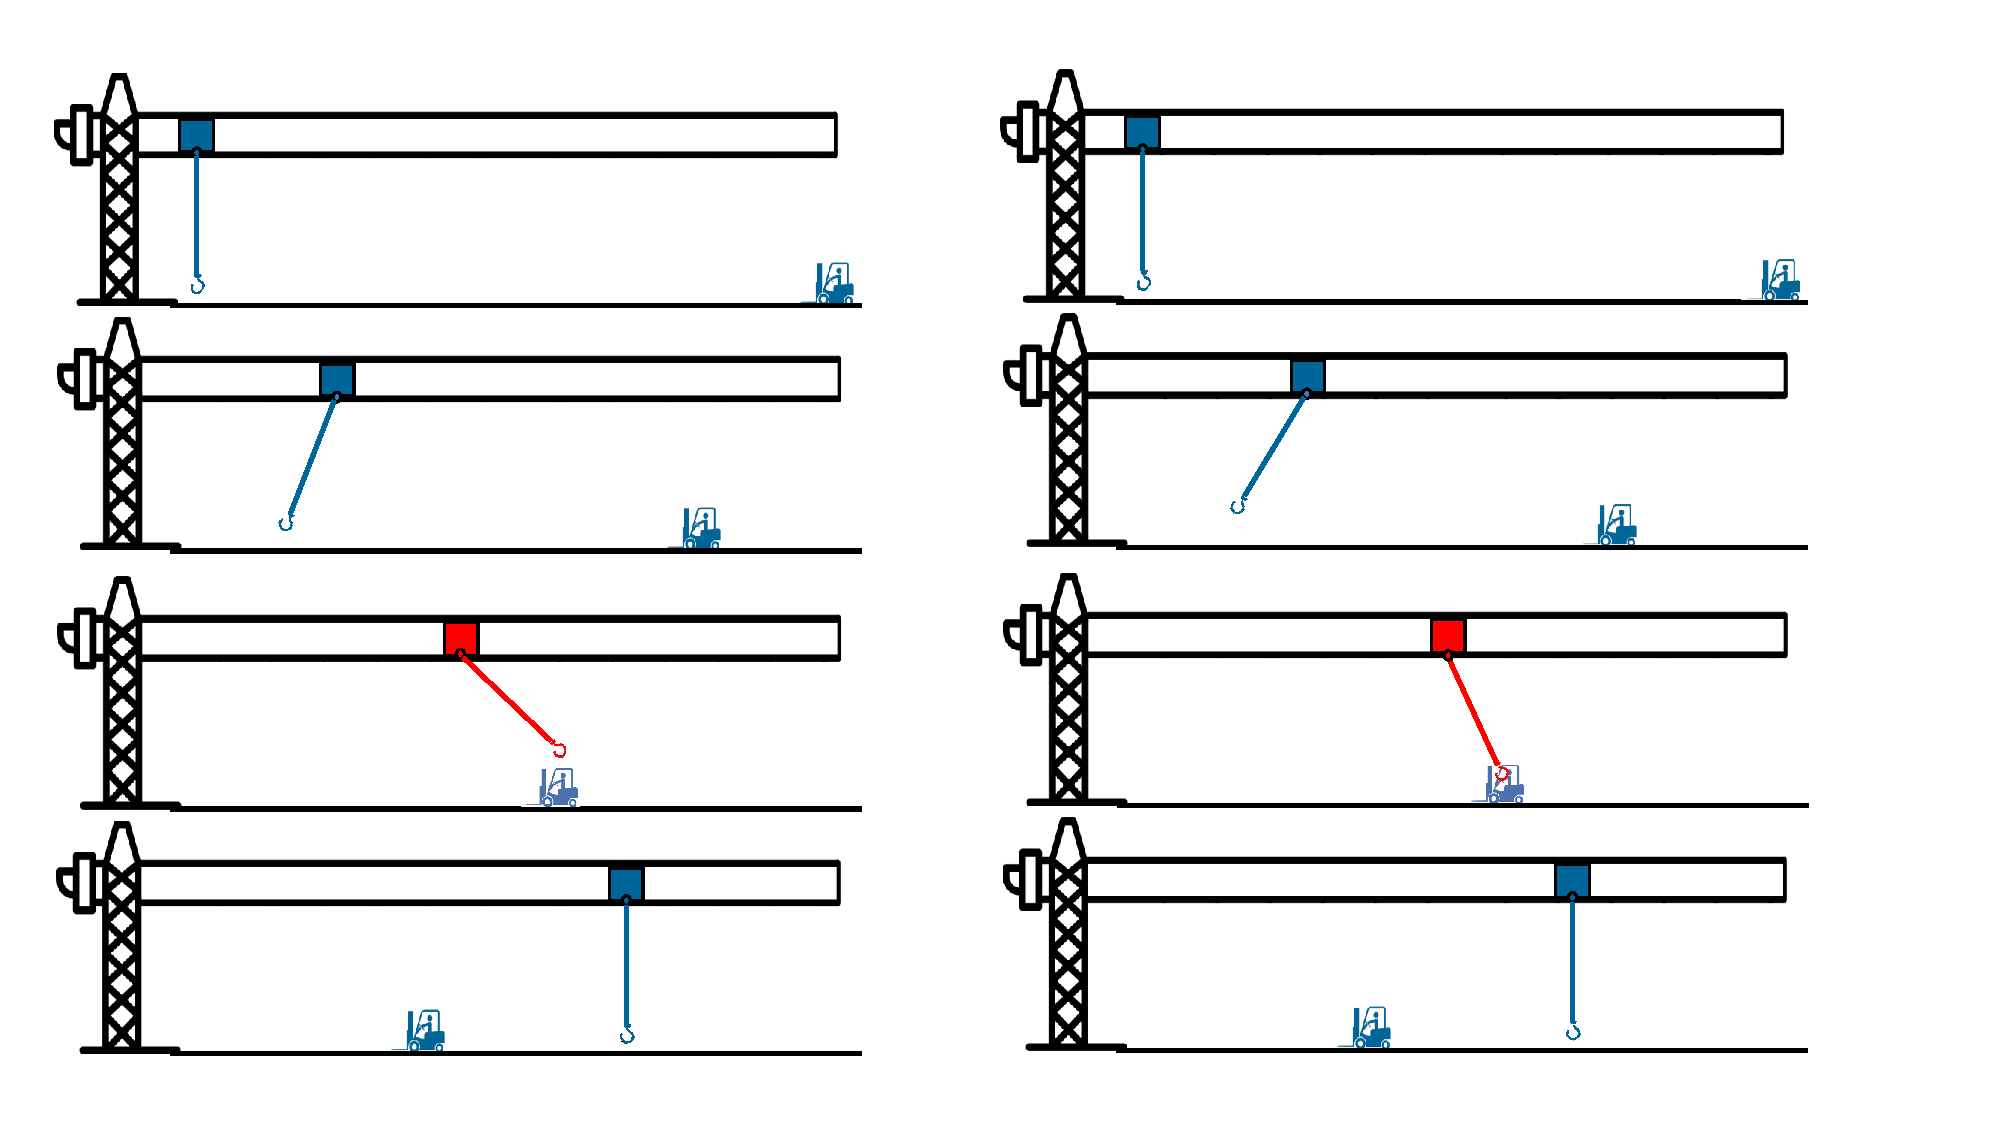
\includegraphics[width=0.45\textwidth]{figures/crane_and_forklifter.pdf}
%	\caption{Illustration of the trajectories generated by the open-loop controller for the crane and vehicle example under disturbance-free (\textbf{left}) and perturbed (\textbf{right}) situations} 
%	\label{fig:cr_and_lft_2}
%\end{figure}


%In this example, we show the method can handle multiple heterogeneous dynamical systems. This example is Modelling a special situation in a factory(shown in fig \ref{fig:cr_and_lft}) . Assume there is a crane and and a forklift. Each one of them should reach their destination without having any accident(satisfying specs). The Crane position will change from 0 to 5 and the forklift from 9 to 4.  Here we model the forklift using $\begin{bmatrix} \dot{x_1}\\ \dot{x_2} \end{bmatrix}=\begin{bmatrix} x_2\\ u \end{bmatrix}$ ($x_1$ and $x_2$ are representing position and velocity) and for the crane we use inverted pendulum model with exactly same configuration in \cite{barto1983neuronlike}: \\ 
%\[\begin{bmatrix}
%\dot{x}\\
%\Ddot{x}\\
%\dot{\theta}\\
%\Ddot{\theta}
%\end{bmatrix}=\begin{bmatrix}
%\dot{x_1}\\
%\dot{x_2}\\
%\dot{x_3}\\
%\dot{x_4}
%\end{bmatrix}=\begin{bmatrix}
%x_2\\
%g(x_3,x_4,u)\\
%x_4\\
%f(x_3,x_4,u)\\
%\end{bmatrix}\]
%
%where $x$ represent position of the cart  and $\theta$ is angle of the pole, f and g are non-linear functions. The process of controller design is similar to Sec. \ref{sec:MultiAgent}; At first we find a nominal trajectory with ALTRO with required specifications then we robustifing it using our method with modified ABCD.\\
%In this example we do not have any static obstacle, but for collision avoidance we use euclidean distance as the metric with $\delta=0.4$ for measuring distance between crane and forklift. We consider hook of crane as a point mass with a radius and forklift as several point mass on circumference of it, So we consider minimum distance between the hook and points of the forklift as the distance. ALTRO solve this trajectory generation problem using sampling time =0.1 and number of points=40 in 10.7 seconds.\\
%to guarantee collision avoidance specification we should select tube sizes to satisfy:
%\[ \delta_{col}> \varepsilon_x + l*\varepsilon_\theta + \varepsilon^\prime_x\]
%where $\varepsilon_x$ and $\varepsilon_\theta$ are tube sizes for position and angle in crane model (cart pole) and l is the length of the joint and $\varepsilon^\prime_x$ is tube size for position of the forklift.
%In next phase we use finite abstraction with $\varepsilon_x=9*0.015$ and $\varepsilon_\theta=11*0.015$ and $\varepsilon^\prime_x=9*0.015$. It takes about 1000 seconds for crane (cart-pole system) with (1.15)*($10^{11}$) number of state-input pairs and ($7*10^6$)*(71) reduced number of states and synthesis takes 35 seconds. For forklift abstractions abstraction and synthesis will finish in less than a second.\\
%The nominal controller with disturbances $w_1=[0,0.02,0,0]$ for crane and $w_2=[0,0.1]$ for forklift will fail collision specification.
%
%


%} 

\begin{figure}
	\centering
	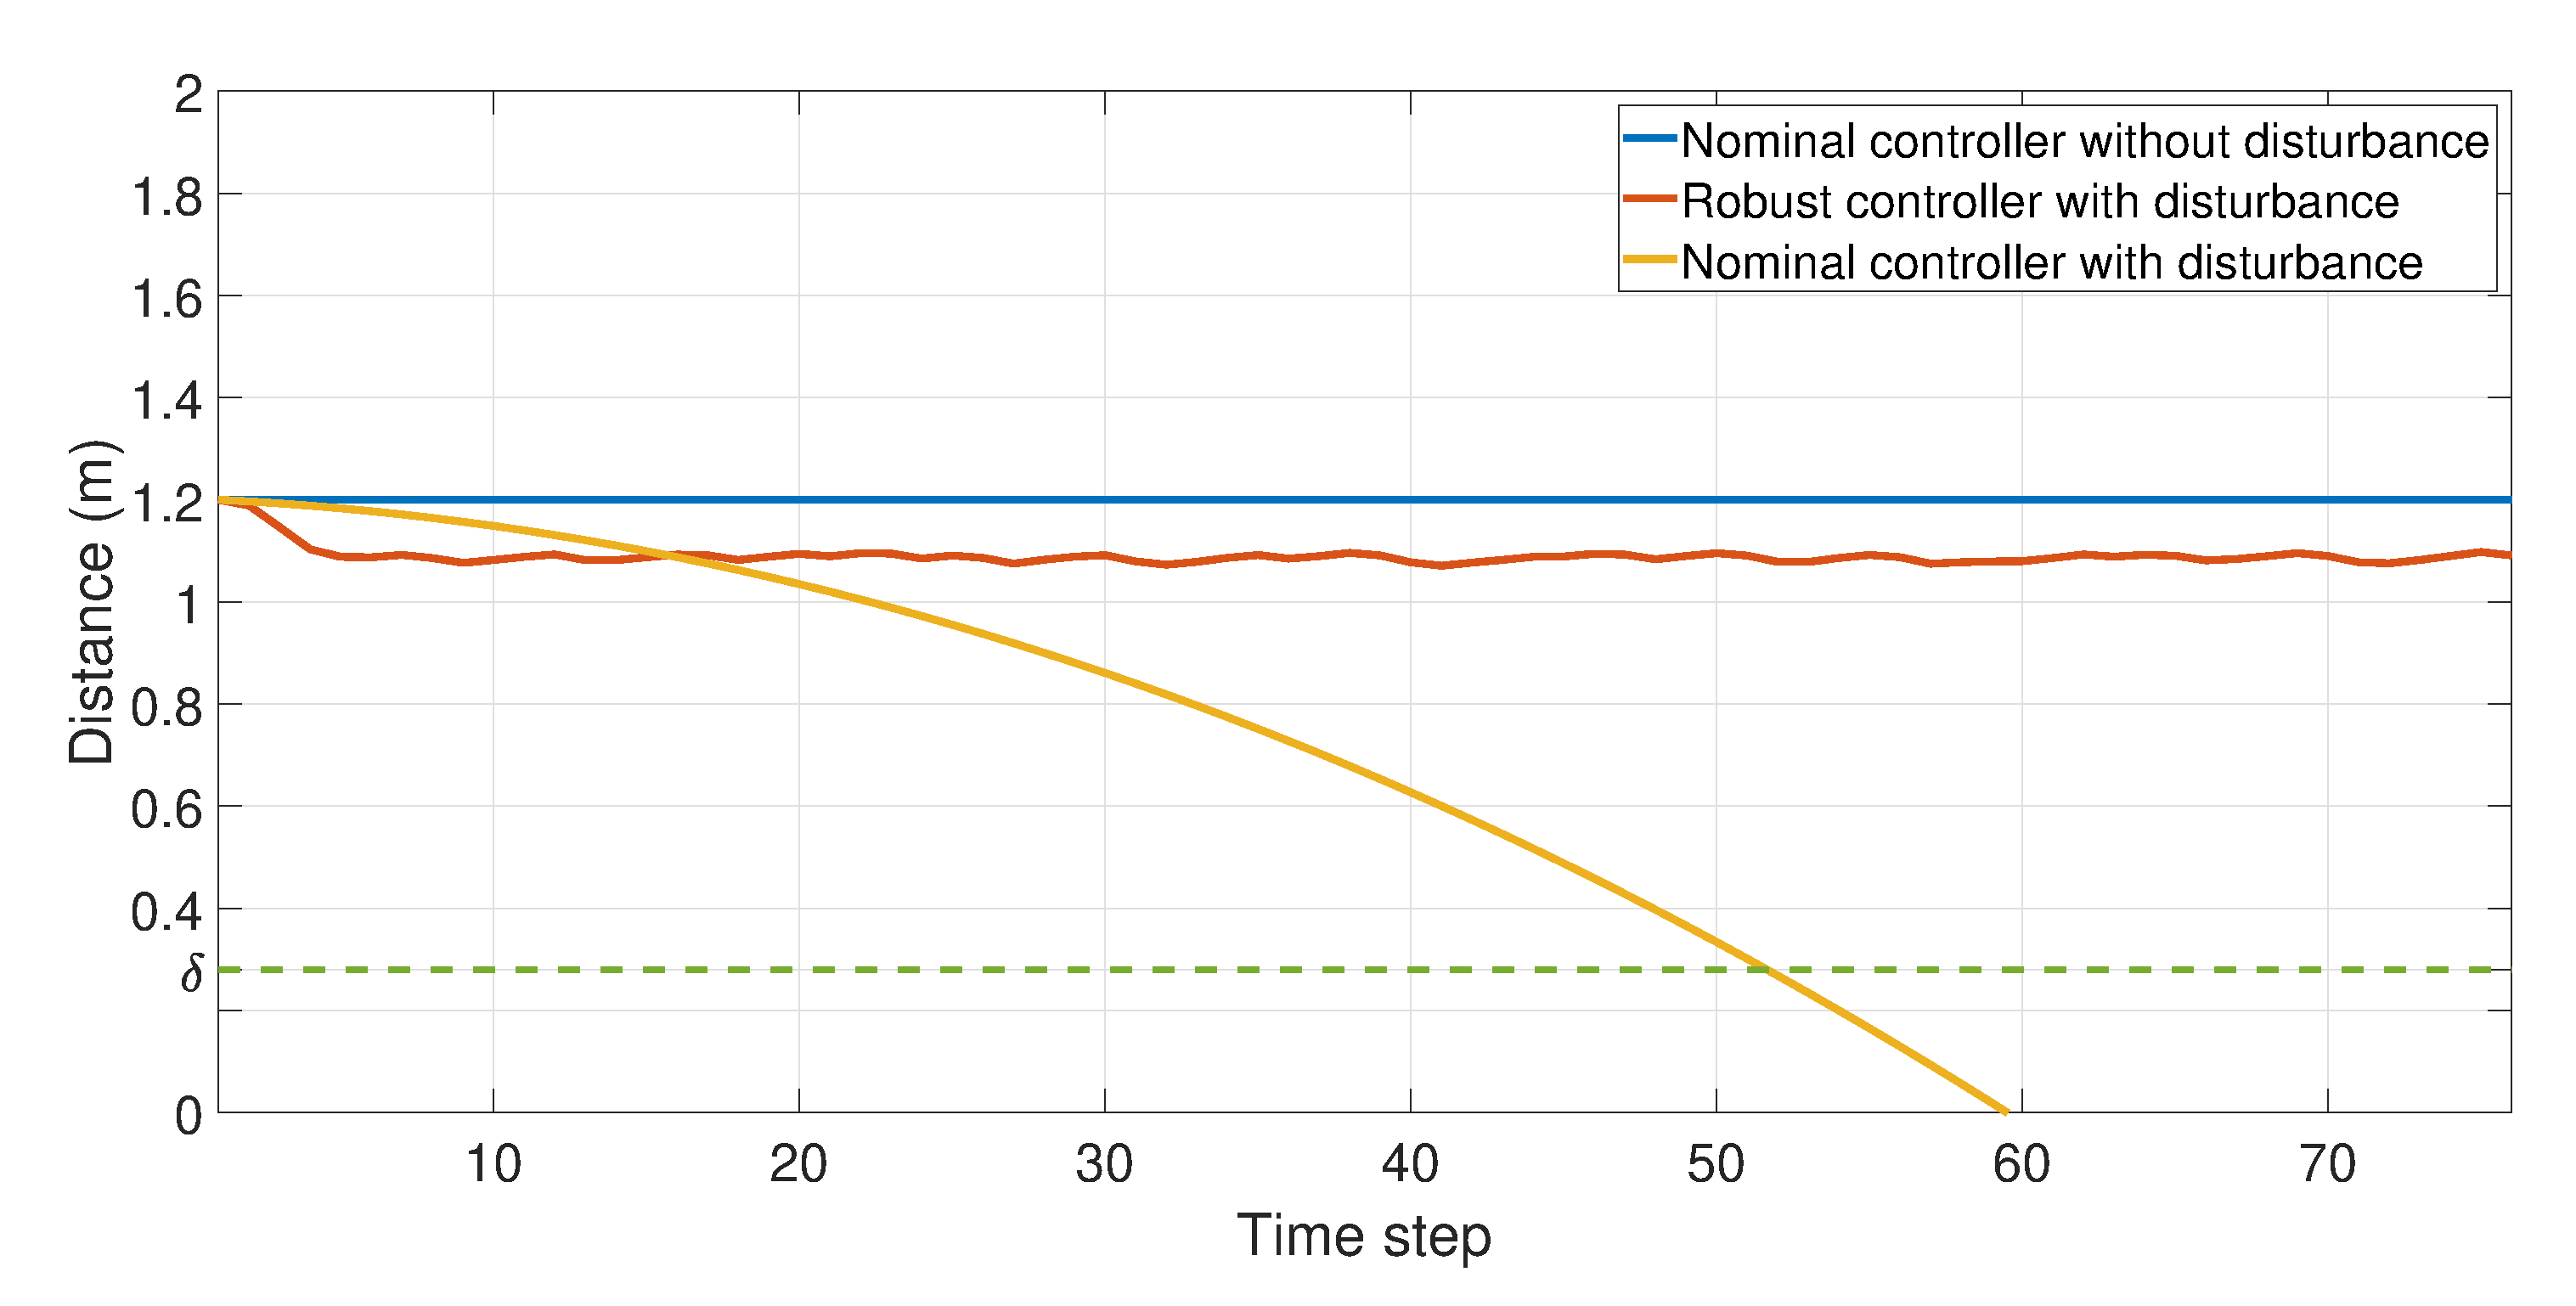
\includegraphics[width=0.45\textwidth]{figures/Merge_plot2.eps}
	\caption{Comparison of open-loop and feedback controllers for the lane merging example}
	\label{fig:merging_distance}
	\vspace*{-0.3cm}
\end{figure}

\subsection{Lane Merging}
\label{sec:lane merging}

%Every vehicle is modeled as tuple $\Sigma=(X,U,W,f^v,Y,h^v)$. 
%Dynamics for each vehicle takes the form
%\begin{equation*}\label{eq:vehicle_ss}
%	f^{v}(x(t),u(t))=
%	\begin{bmatrix}
%		\dot{x_1}\\
%		\dot{x_2}
%	\end{bmatrix}=
%	\begin{bmatrix}
%		u_1\\
%		u_2
%	\end{bmatrix},
%\end{equation*}
%where $x_1$, $x_2$ denote the vehicle's position in $2D$ plane, $u_1$ and $u_2$ represent the vehicle's speed coordinates, respectively. The output mapping is defined as
%\[
%h^v(x(t))=x(t).
%\]
The nominal dynamics for each of the vehicles is the same as the one  for modeling drones (given in Sec.~\ref{sec:Multirobot}). 
The disturbance set and robustness margin are chosen as $|W|\leq (0.03,0.03,0.03)$ and $\varepsilon=(0.16,0.16,0.16)$. %($\Sigma^i=(X,x_\init^i,U,W,f^d_\tau)$). 
For collision and obstacle avoidance, we choose $\delta=0.37$.
The horizon length is fixed to $T=110$. 
Given these settings, ALTRO generates a valid nominal trajectory in $89.02$ seconds. 
Next, we use ABCD in order to compute feedback controllers tolerating additive disturbance $W$. 
We choose state and input spaces for each vehicle's model to be $X=[-0.5,15]\times[0.1,7.4]\times[-1,0.4]$ and $U=[-0.9,3]\times[-2.1,2.1]$, respectively. 
State and input partition sizes are chosen as $\eta_{X}=(0.02,0.02,0.02)$ and $\eta_{U}=(0.3,0.15)$. 
Tab.~\ref{tab:runtimes} shows run times and number of state-input pairs corresponding to local and global ABCD. 
For $N>1$, memory requirement for global ABCD exceeds memory limits.
Fig.~\ref{fig:merge} demonstrates snapshots of one sample trajectory when feedback controllers are employed under the presence of disturbance. It should be noticed that using ALTRO alone would not provide guarantee against bounded disturbance.
Fig.~\ref{fig:merging_distance} illustrates the fact that open-loop controller fails in keeping one of the vehicles away from the road's sides under perturbed situation when constant additive disturbance vector $(-0.03 ,0.03,-0.03)$ is being applied throughout the whole horizon. 
In contrast, employing a feedback controller results in successful lane merging. 





\begin{figure}[t]
	\centering
	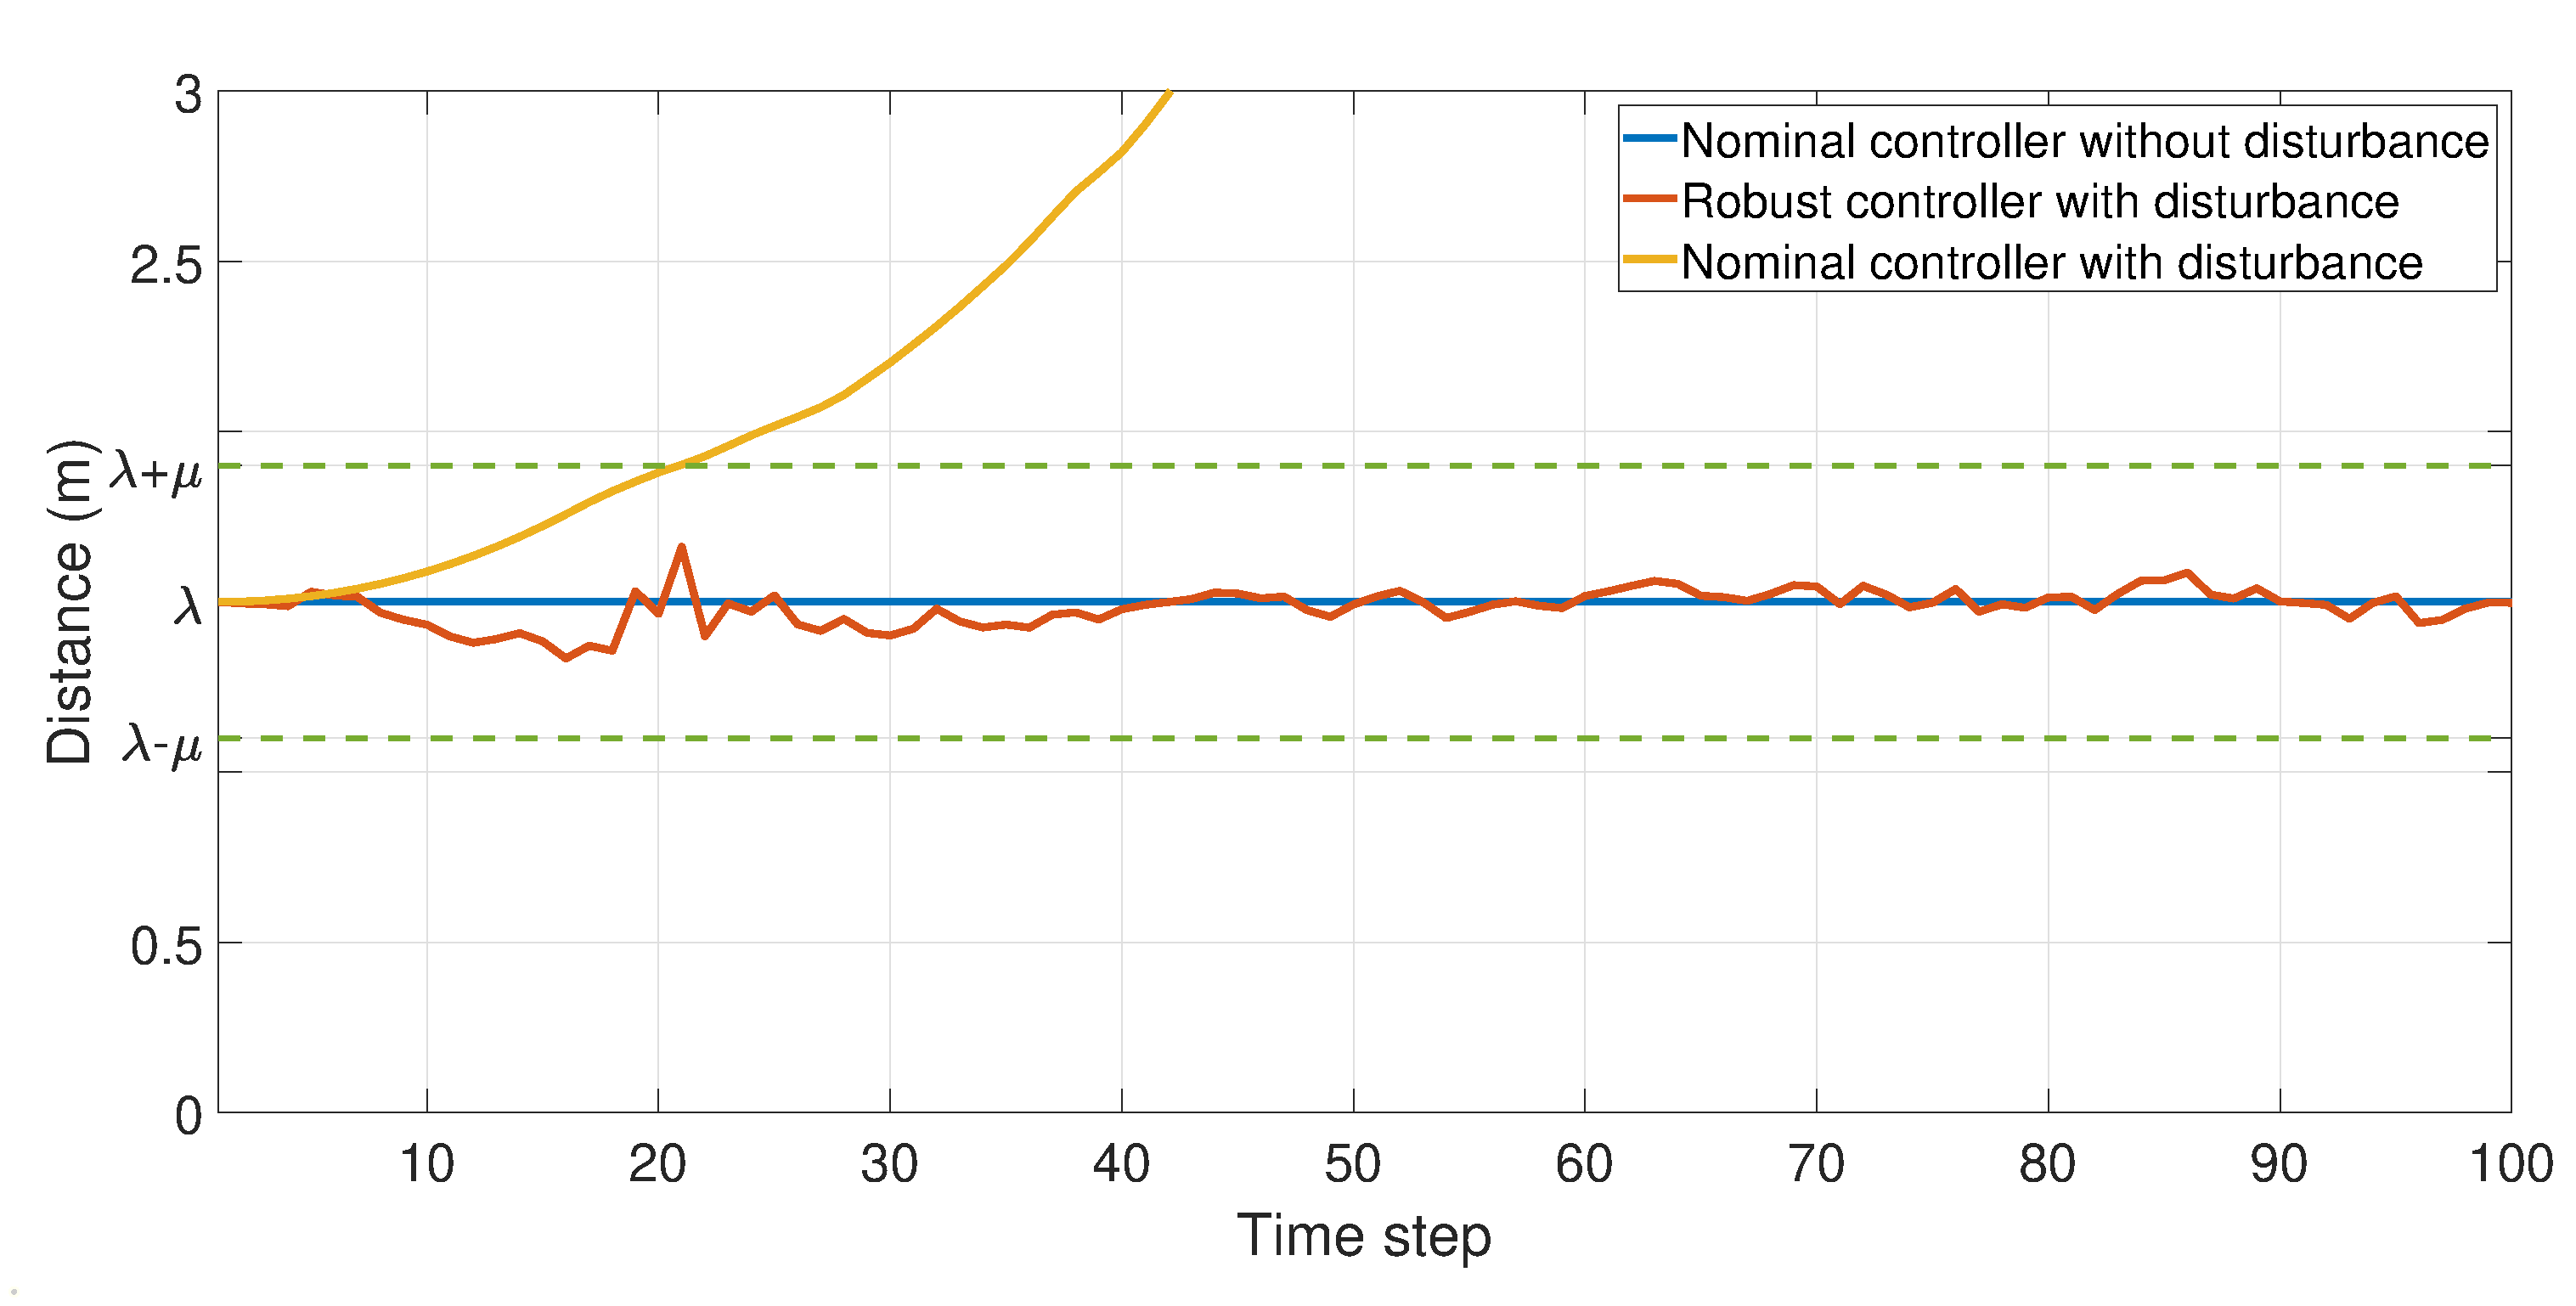
\includegraphics[width=0.45\textwidth]{figures/formation_dist2.eps}
	\caption{Comparison of open-loop and feedback controllers for the formation control example}
	\label{fig:formation_distance}
	\vspace*{-0.5cm}
\end{figure}

\subsection{Multi-drone formation control}
\label{sec:formation_control}

In the multi-drone formation control case study, the nominal dynamics for each of the drones is the same as that in 
Sec.~\ref{sec:Multirobot}. 
The disturbance set and robustness margin are chosen as $|W|\leq (0.03,0.03,0.03)$ and $\varepsilon=(0.24,0.24,0.24)$. 
Distance between each pair of drones positioned at the diamond's vertices is set to be $\lambda^{i,j}=\frac{3\sqrt{2}}{2}$ 
for $i,j\in\set{1,2,3,4}$, while the drone positioned at the center is supposed to keep distance $\lambda^{5,j}=1.5$ 
for $j\in\set{1,2,3,4}$. 
Setting the minimum distance for obstacle avoidance to $\delta=0.4$ and horizon length $T=100$, 
ALTRO finds a valid solution over the product system with $15$ state and $10$ input variables within $114.3$ seconds.
Next, we synthesize local controllers for every drone such that the specifications hold for the perturbed models with $\mu=0.5$. %We construct a tube around the (nominal) trajectory produced by ALTRO with the width vector $\varepsilon=\begin{bmatrix}??&??&??\end{bmatrix}^T$.
%\RM{the state space should go before ALTRO}
We consider state and input spaces to be $X=[-2,17]\times[-2,17]\times[0.6,1.6]$ and
$U=[-0.9,4.8]\times[-3,3]$, respectively. We select $\eta_{X}=(0.03,0.03,0.03)$ and
$\eta_{U}=(0.3,0.15)$. % and $\varepsilon=\begin{bmatrix}0.18&0.18&0.18\end{bmatrix}^T$.% results in state and input spaces with $10^9$ and $820$ points. 
%Computing the transition system over inter-tube space with width $\varepsilon=\begin{bmatrix}0.18&0.18&0.18\end{bmatrix}^T$ results in smaller transition system with $4.9\times 10^5$ points. Given the above settings, SCOTS computes abstraction in $271$ seconds ($54.2$ seconds in average) and $66.5$ seconds ($13.3$ seconds in average). 
Tab.~\ref{tab:runtimes} shows the run times and number of state-input pairs corresponding to local and global ABCD. 
Already for two drones, the memory requirement for global ABCD exceeds the available memory of 1.5TB of RAM.
Fig.~\ref{fig:formation_ex} illustrates four sequential frames of a sample perturbed trajectory generated by employing 
feedback controllers. Notice that both 
relative position and orientation between drones are kept (almost) constant 
throughout the journey. 
On the other hand, using ALTRO alone would not provide guarantee against bounded disturbance. 
Fig.~\ref{fig:formation_distance} illustrates performance of open-loop and feedback controllers on regulating distance between two specific 
drones with and without disturbances. 
As expected, in the absence of disturbances, the open-loop controllers suffice and the distance between the two drones 
(shown in solid blue) does not go below the threshold line (showed as the dotted line). 
However, when constant additive disturbance vectors 
$(0 ,0.03,0.03)$ and $(0 ,-0.03,-0.03)$
are being applied to the two drones throughout the whole horizon, open-loop controller fails, 
whereas the feedback controller is still capable of maintaining distance above the given threshold.

